\documentclass[11pt,a4paper]{article}
\bibliographystyle{apalike}
\usepackage{amssymb}
\usepackage{epsfig}
\usepackage{amsmath}
\usepackage{natbib}
\begin{document}

\section{Introduction}
{\bf TO DO: Beef this up, but not necessarily by much}
Why you care about BHs... all the usual reasons, \\
good tests of extreme astrophysics,  \\
SMBHs tied to gal formation \\
SMBHs let you have quasar backlights for Ly$\alpha$-forest\\

Why you care about RVM... \\

Why you care about photometric RVM \\

(this will naturally be pretty close to the intro for the
Chelouhce paper...) 

{\bf N.B. make some sort of compare and contrast to Chelouche12...; 
e.g. PG QSOs vs. S82 quasars; epochs, $z$-range etc.}

\subsection{Reverberation Mapping Basics}
Peterson etc. discussion... (two or three review articles to read/quote here...)
After emission-line variability was detected, it became possible to
think that the kinematics and the geometry of the BLR can be tightly
constrained by characterizing the emission-line response to continuum
variations. The time delay between continuum and emission-line
variations are ascribed to light travel-time effects within the BLR;
the emission lines ``echo'' or ``reverberate'' to the continuum
changes. The Blandford \& McKee paper, regarded as the seminal paper
in the field, first introduced the term ``reverberation mapping'' to
describe this process. Reviews of progress in reverberation mapping
are provided by Peterson and Netzer \& Peterson.

\smallskip
\smallskip
\noindent
From Barth et al. (2011ApJ...743L...4B; http://arxiv.org/abs/1111.0061v1)::

\smallskip
\smallskip
\noindent
By measuring the time delay between AGN continuum variations and the
subsequent response of the broad-line region (BLR) gas, the
light-travel time across the BLR, and hence the mean BLR radius
($r_{\rm BLR}$), can be directly measured.

\smallskip
\smallskip
\noindent
With a direct measurement or estimate of $r_{\rm BLR}$ , and assuming
virial motion of BLR clouds, it becomes possible to estimate the mass
of the black hole in an AGN as:
\begin{equation}
M_{\rm BH} = f\cdot  r_{\rm BLR}(\Delta V)^{2}/G	
\end{equation}
where is the width of the broad line, and f is a dimensionless scaling
factor (e.g., Ulrich et al. 1984; Kaspi et al. 2000; Onken et
al. 2004). This method has been used to estimate black hole masses in
large samples of AGNs out to the highest observed redshifts (for a
review, see Vestergaard 2011).

\subsection{Kinda of observations you could enivage}
{\bf TO DO: Again, beef this up, but not necessarily by much}
Now that we've described (p)RVM, here are the general 
considerations for the types of observations one might want/need...
(even be a bullet list??)

Okay, these are kinda the observations {\it you want...}
and this naturally segues into...




\section{Data}
SDSS S82. 
(Huff reference...; Ross reference...)
Palanque-Delabrouille11, Fig 12  \\
{\bf TO DO: Fig 12 Palanque-Delabrouille et al. (2011)  equivalent}\\

Which SDSS DR$x$ paper gives the photo and spectra table meanings..
photoObj and specObj descriptions... (Stoughton et al.???!) 

``Dream table'' of lots of quasars with lots of photo-epochs.\\
{\bf TO DO: NPR to ``stress-test'' this file/catalog}

In another note, how do we display the data, with its natural cadence,
of lots of information on short t-scales and year-long t-scales.  And,
how will this translate/affect our measurements (e.g. biases on these
periods...)

    \subsection{Sample Selection}
    e.g. drop/investigate BAL QSOs...
    
    
    
\section{Method}
Follow again Chelouche12 closely. \\
Chelouche12+binning scheme+ more sophisticated model for the QSOs.


   \subsection{Cross-correlation Basics}
   %% Mainly from wikipedia; mainly for NPRs benefit...
   I have a signal that is just Gaussian White Noise:
   \begin{equation}
     f(t)=\frac{1}{\sigma\sqrt{2\pi}}\exp^{-\frac{1}{2}(\frac{t-\mu}{\sigma})}     
   \end{equation}
  \begin{equation}
    g(t+\tau)=\frac{1}{\sigma\sqrt{2\pi}}\exp^{-\frac{1}{2}(\frac{[t+\tau]-\mu}{\sigma})}     
  \end{equation}
  Now a cross-correlation is: 
 \begin{equation}
   (f \star g)(t) = \int^{\infty}_{-\infty} f^{*}(\tau) \ g(t+\tau) \ d\tau
 \end{equation}
 where $f^{*}$ is the  complex conjugate of $f$, i.e. 
  \begin{equation}
    f^{*}(t)=\frac{1}{\sigma\sqrt{2\pi}}\exp^{\frac{1}{2}(\frac{t-\mu}{\sigma})}     
 \end{equation}
 Thus, 
 \begin{eqnarray}
  (f \star g)(t) & = & \int^{\infty}_{-\infty} f^{*}(\tau) \ g(t+\tau) \ d\tau \\
                     & = & \int^{\infty}_{-\infty}  \frac{1}{\sigma\sqrt{2\pi}} \exp^{\frac{1}{2}(\frac{t-\mu}{\sigma})}     
                                                             \frac{1}{\sigma\sqrt{2\pi}} \exp^{-\frac{1}{2}(\frac{[t+\tau]-\mu}{\sigma})}     \\
                      &= & \frac{1}{2\pi\sigma^{2}}   \int^{\infty}_{-\infty}  \exp^{\frac{1}{2}(\frac{t-\mu}{\sigma})}   \exp^{-\frac{1}{2}(\frac{[t+\tau]-\mu}{\sigma})} \\
                      & = & ....
 \end{eqnarray}
 
 \subsubsection{What we actually try to measure}
 Measuring the cross-correlation of the various SDSS light curves is
 the first step, but it is not, in itself, Science. The physically
 meaningful information about the accretion disk size and geometry is
 compressed into the transfer function, $\psi(t)$. The transfer
 function is the kernel of the linear mapping between the continuum
 and emission line light curves. Letting $C(t)$ be the continuum light
 curve, and $L(t)$ be that of the emission lines:
 \begin{equation}
   L(t) = \int_0^{\infty}\,dt'\,\,C(t') \psi(t'-t)
 \end{equation}
 Normally for these problems we think of $\psi$ as being peaked at
 $t\geq 0$, which creates the time lag, and as having some finite
 width, which is a result of
 averaging the response to variations in the black hole accretion rate
 over the physically much larger geometry of the broad-line emitting
 region [REF: e.g., Blandford \& McKee 1982].
 
 So we can think of the measurement problem here as being one of
 extracting as much information about $\psi$ as is possible, given a
 set of noisy lightcurves. This section describes the derivation of an
 {\it optimal quadratic estimator} (the OQE) for $\psi$. To begin with, we'll
 imagine binnning the continuous $\psi$ into a discrete histogram with
 constant bin widths $w$ and histogramed values $\psi_m$. If
 $\Omega(t-t_m;w)$ is a unit-area top hat of width $w$ covering the
 area around $t=t_n=nw$, then the transfer function can be written as:
\begin{equation}
  \psi = \sum\limits_{m=0}^{N_{\rm bins}}\psi_m\Omega(t-t_m;w)
\end{equation}
This is a flexible and intuitive parameterization of any functional
form of $\psi$, and having chosen a useful parameterization, we can
now do statistics.

What we seek is the minimum-variance estimator for the vector $\psi_m$
given a discrete sampling of two light curves $C(t_i)$ and
$L(t_i)$\footnote{Note that the sampling times $t_i$ need not at this point
have anything at all to do with the locations of the transfer function
bins $t_m$.}.

If we can express the signal covariance matrices of the light curves,
$S_{CC}$, $S_{LL}$, and $S_{CL}$ as a function of our desired
parameters $\psi_m$, we can look up the answer (the OQE for $\psi_m$)
in any one of several power-spectrum estimation papers [REF:e.g.,
Seljak 1998, Tegmark 1997, etc.]. The minimum variance estimator for
our parameters $\hat{\psi}$ is: \begin{equation}
  \hat{\psi}_m = \sum\limits_{n}\left(F^{-1}\right)_{mn}\left(q_n-f_n\right)
\end{equation}
where $F$ is the Fisher matrix, and the other quantities $q$ and $f$
are written in terms of the covariance matrices as:
\begin{align}
  F_{mn} &=\frac{1}{2}{\rm Tr}\left[\mathbf{C}^{-1}\mathbf{C}_{,m}\mathbf{C}^{-1}\mathbf{C}_{,n}\right] \\
  q_n &=\frac{1}{2}{\rm Tr}\left[\mathbf{C}^{-1}\mathbf{C}_{,n}\mathbf{C}^{-1}\mathbf{N}\right] \\
  f_n &=\frac{1}{2}\mathbf{y}^{\rm T}\mathbf{C}^{-1}\mathbf{C}_{,n}\mathbf{C}^{-1}\mathbf{y}.
\end{align} {\it Note: that I simply copied this expression from
  Jordan Carlson's notes on optimal bandpower estimators for power
  spectra. A proof is supplied therein, and the above result can be
  found in many cosmology papers. The implications for analyzing
  generic, inhomogenously sampled timeseries do not seem to be
  appreciated yet in the literature, as far as I can tell.} Here,
$\mathbf{y}$ is the full data covariance matrix (think of this as
making a single long vector from the two measured timeseries $C(t_i)$
and $L(t_i)$). $\mathbf{C}$ is the full covariance of this vector, and
the $\mathbf{C}_{,n}$ notation is meant to indicate the derivative of
the covariance matrix with respect to the $n^{\rm th}$ parameter we
are trying to measure -- in our case, $\psi_n$. This is why it's
useful to write $\psi$ in a discretely parameterized form.

The first task in deriving $\hat{\psi}$ is calculate the covariance
matrix $\mathbf{C}$. There are three steps here. The covariance matrix
$S_{CC}=cov\left(C(t_i),C(t_j)\right)$ of the continuum timeseries is
easy; we fixed this when we assumed the DRW form of the quasar power
spectrum. The covariance matrices
$S_{LL}=cov\left(L(t_i),L(t_j)\right)$ and
$S_{CL}=cov\left(C(t_i),L(t_j)\right)$ are also both analytically
calculable once the noise properties of the continuum are determined.

TODO: Finish calcluating $\mathbf{C}_{,n}$, and derive the OQE. We can
test its performance on the data. This turns out to be just repeated
application of the convolution theorem, plus some numerical
integration.

TODO: Write down the covariance matrix $cov\left(\psi_m,\psi_n\right)$.
Again, this is something we can just look up, and in the same places
as the above.

TODO: Once we know the binned $\psi_n$ estimator in bins, we can
immediately write down the estimator for a linear combination of those
bins (this is in the Seljak paper). This is cool, because we can then
do calculus -- let the bin widths that define $\psi_m$ go to zero, and
pick some finite-width filtered $\psi$ to be the thing that we
actually estimate. This is nice because it lets us play around with
the binning scheme without worrying about smoothness conditions on
$\psi$, and it neatly resolves the tension between generality ($w<<1$
so that we can represent any $\psi$) and practicality ($w>>1$, since
our data is noisy and we'll probably only really be able to get $\psi$
in fat time bins.

TODO: Demonstrate the performance of the estimator on the simulations.
This is the easy part.

    \subsection{Binning Scheme and Scaling Relations}
    How some BLACK HOLE MASS in some binning, relates to {\it something}
    Luminosity, bulge size, or just   {\it something}...
    

    \subsection{QSO model}
    Chelouche12 just assume EWs and variability time-scales. 
    We have to be smarter since we have a (much) broader $z$-range
    and $L$ and Mass range...
    
    Bit more, since we're going to have to describe our binning scheme...\\
    
    \subsection{Errors}
    Misra et al. (2010) 

    \subsection{Fitting+Simulations...}
    Some sort of model, some sort of data $\Rightarrow$ fitting... \\
    Worry about: 
    \begin{itemize}
      \item{Aliasing}
      \item{noise biases} 
      \item{other stuff in terms of systematics we haven't though of...}
    \end{itemize}
    How can we figure out what out biases are...

    \subsection{Simulations}
    To make simulated quasar light curves, we start by assuming we
    know something about the variability. Certain authoritative
    sources (REF=???) characterize quasar variability as a ``damped
    random walk'', or ``brownian noise''. This turns out to be a
    sampling of a random process with a noise power spectrum $P(\omega)$
    such that:
    \begin{equation}
      P(\omega) = S_0/\omega^2
      \label{eqn:BrownNoise}
    \end{equation}
    It turns out that this is really easy to generate, if you can make
    normally-distributed random numbers. The two key properties of real, gaussian
    scalar fields are that:
    \begin{itemize}
    \item The phases of their Fourier transforms have odd symmetry.
    \item The deterministic part of the field is completely fixed by
      the power spectrum.
    \end{itemize}
    The power spectrum is just the square of the absolute value of the
    Fourier mode amplitudes. Each Fourier mode consists of a phase and
    an amplitude, so to make a noise realization with a particular
    power spectrum, we need only fix the complex phases and set the
    amplitudes according to equation~\ref{eqn:BrownNoise}. The inverse
    FFT returns a real scalar field with exactly the right noise
    properties.
    
    An example of this process is shown in
    figure~\ref{fig:SampleLightCurves}. The continuum light curve
    $C(t)$ is generated as described above. The line emission $L(t)$
    is generated by convolving the continuum with a gaussian transfer
    function, shifted by a small lag $\tau$ relative to the emission:
    \begin{equation}
      L(t) = \int_{0}^{\infty}C(t')\Psi(t'-\tau)\, dt'
    \end{equation}
    [REF: Peterson 199X]. This has the effect of smoothing the
    continuum light curve and shifting it by $\tau$.
    
    \begin{figure}
      \begin{center}
        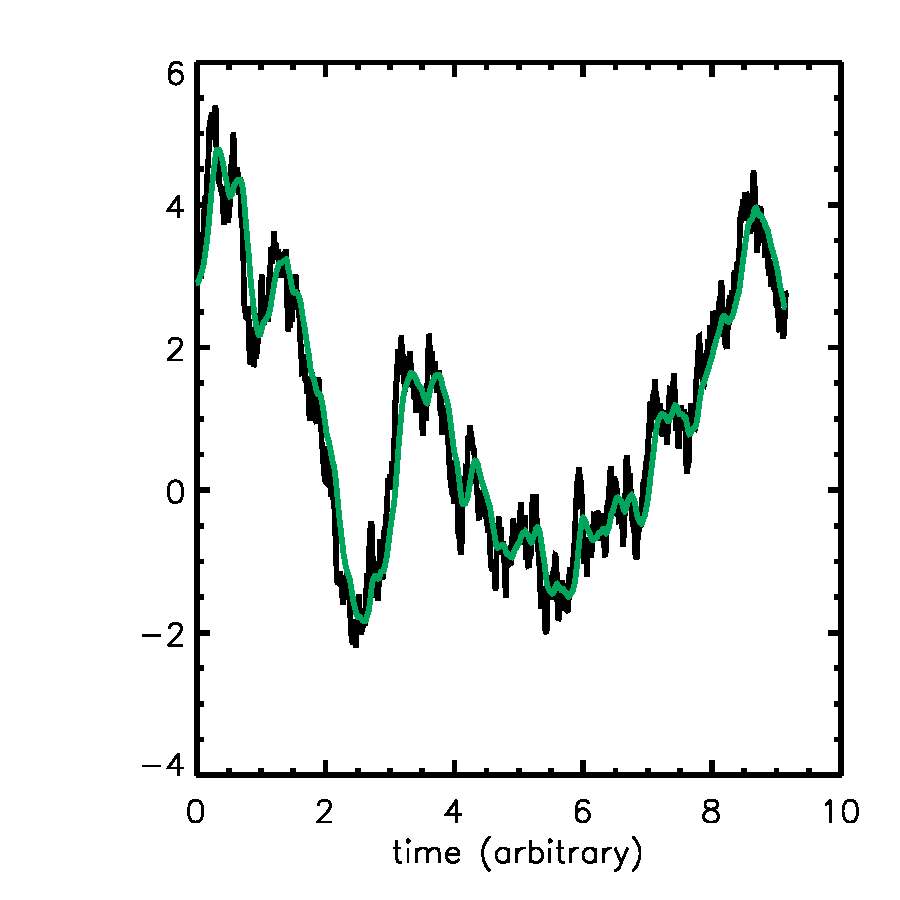
\includegraphics[width=4in]{../Plots/sample_lightcurve.pdf}
        \caption{Two light curves, meant to represent the time
          variability of the continuum (black) and broad emission-line
          (green) features.}
        \label{fig:SampleLightCurves}
      \end{center}
    \end{figure}
    
    The time-varyong component observed in each filter will be a
    linear combination of some line emission and some continuum
    emission. We could use a quasar template spectrum and the SDSS
    filter curves (which are very well known... right???) to model
    this.

    Also important to keep in mind is that the characteristic
    timescale of variation is reduced with redshift, as $t-\tau
    \mapsto \frac{t-\tau}{1+z}$, and that $\tau$ is thought to scale
    with a low power of the intrinsic quasar luminosity.
    
    This strongly suggests we should bin our objects by luminosity and
    redshift, at least initially.

      
\section{Results}
     
$\blacktriangleright$ idea: correlation vs. time-lag, but for
different luminosity (or whatever) bins/ranges... General idea, see
a/the peak of the CF move to different times as a funciton of BH mass
(and whatever we think is tracking BH mass e.g. luminosity bins)

$\spadesuit$
Second plot, BH (or even bulge???!), or a luminosity vs. a $\Delta t$ (what you
classically measure from RVM). 

(Magorrian at $z\sim1$ ???!!!!) 

$\pounds$\footnote{These are the money plots, right?}

$\spadesuit$Comparison on
NGC 4395...

$\spadesuit$Comparison/killer plot along the 
e.g Figure 14 of MacLeod et al. (2010), ApJ, 721, 1014.


\section{Discussion}

    \subsection{Issues arrising...}
    Knowing where this is soft... 
    (key issue for NPR). 
    First thing: the time-delay is acutally from BH mass, due to e.g. geometry...
    - what the {\it f-is-f}...

    - If I'm designing my ideal survey, in light of these (data)
    results, and potentially tests from our simulations, how would I do
    it...??  (this can link back very nicely to the discussion in the
    Intro...)
    
    \subsection{Viewing angle...}
    Can you bin by constant viewing angle...
    Does it have no affect on variability...
    The Croom/Fine paper (NPR to look out 

    \subsection{Dream World...}
    (When we are designing our polarization survey... :-) 


\section{General}
E.H. Want to be able to write down a model for quasars...
List of observables and theoretical quantatites...
draw the arrows between them...
mapping between concepts and the model - tells you what
 to test...
Bigger Picture: the broad-framework for QSOs...
(cutting edge-stats etc.) and it tells us what to do
(prescriptive). 

How quasars work; Boxes and arrows...



\end{document}
